\chapter{Evaluaci\'on experimental}

En este cap\'itulo presentamos los resultados de ejecutar el algoritmo de b\'usqueda por rango usando dos t\'ecnicas de selecci\'on de pivotes: aleatoria y incremental.\\

Comenzaremos describiendo el seteo experimental, los experimentos realizados y luego daremos el an\'alisis de los resultados obtenidos.\\

\section{Seteo Experimental}

Como mencionamos anteriormente, para los experimentos presentados en \'este cap\'itulo utilizamos los productos (\textit{items}) publicados en la plataforma de e-commerce Mercado Libre, divididos en 30 categor\'ias.\\

\subsection{Elecci\'on de la cantidad de pivotes y agrupaci\'on de categor\'ias}
El hecho de que la cantidad de elementos de las categor\'ias estuviera distribu\'ido en un rango muy amplio (de 1034 elementos para la categor\'ia m\'as peque\~na a 213578 elementos para la catego\'ia m\'as grande), nos oblig\'o a segmentar dichas categor\'ias en 4 grupos de acuerdo a su tamaño.\\

En base a \'este mismo criterio, realizamos la elecci\'on de la cantidad de pivotes, teniendo en cuenta el porcentaje que los mismos representaban sobre el total de los items de cada categor\'ia. La distribuci\'on resultante se presenta en la siguiente tabla:\\

\begin{table}[htbp]
\begin{center}
\begin{tabular}{|p{1.1cm}|p{1.8cm}|p{3.2cm}|p{2.2cm}|p{2.5cm}|}
\hline
Grupo & 
Cantidad de Categs & 
Rango del tama\~no & 
N\'umero de Pivotes \\
\hline \hline
1 & 
6 & 
[1.034 - 15.964] & 
16, 32, 64, 128, 256  \\ \hline
2 &
12 &
[19.032 - 46.530] &
64, 128, 256, 512, 1024  \\ \hline
3 &
8 &
[57.198 - 13.6323] &
256, 512, 1024, 2048  \\ \hline
4 &
4 &
[16.7995- 21.3578] &
512, 1024, 2048, 4096  \\ \hline
\end{tabular}
\caption{Tabla de grupos.}
\label{tabla:grupos}
\end{center}
\end{table}


\subsection{Selecci\'on del rango de b\'usqueda}

La mayor\'ia de los trabajos de investigaci\'on existentes sobre b\'usqueda por similitud en textos, utilizan como universo de datos diccionarios de palabras como por ejemplo ingl\'es o español. Esto genera una base com\'un que puede utilizarse a la hora de generar variaciones sobre algoritmos de b\'usqueda en nuevos trabajos, es decir, se comparte la base de datos y los par\'ametros de los experimentos, lo cual permite comparar f\'acilmente los resultados de los mismos entre s\'i.\\
 
Es com\'un encontrar trabajos de b\'usqueda por rango donde la variaci\'on del radio es siempre entre 1 y 5 y la elecci\'on de ese valor no requiere m\'as que una simple decisi\'on azarosa por parte del autor.\\

En nuestro trabajo, el universo de datos es bastante m\'as singular, ya que se trata de t\'itulos de productos reales, cuya redacci\'on est\'a a cargo del usuario que publica el producto para su venta y donde la \'unica limitante es el tama\~no de ese t\'itulo (60 caracteres).\\

Esta particularidad tiene como consecuencia un universo de datos variado y heterog\'eneo, donde cada elemento de dicho universo es una combinaci\'on de palabras, abreviaciones, n\'umeros y caracteres especiales. Ante \'esta combinaci\'on de caracter\'isticas, el primer obst\'aculo que debimos sortear para comenzar con la evaluaci\'on experimental fue, precisamente, la selecci\'on del radio de b\'usqueda.\\

Para realizar una primera aproximaci\'on al radio de b\'usqueda ideal, seleccionamos 4 t\'itulos de productos (cuadro \ref{tabla:muestra-rank}) de la categor\'ia con mayor cantidad de elementos (cuadro \ref{tabla:muestra-tamano}) y luego procedimos a realizar una b\'usqueda de los k-vecinos con las siguientes variaciones:\\

\begin{itemize}
\item $k= 0.001 \times  cantidad\_de\_elementos\_de\_la\_categoria\ (0.1\%)$
\item $k= 0.01 \times cantidad\_de\_elementos\_de\_la\_categoria\ (1\%)$
\item $k= 0.1 \times cantidad\_de\_elementos\_de\_la\_categoria\ (10\%)$
\end{itemize}

Las b\'usquedas se realizaron utilizando la estrategia de selecci\'on de pivotes incremental, y la cantidad de pivotes elegida fue de 128.\\

\begin{table}[H]
\begin{center}
\begin{tabular}{|c|c|c|c|}
\hline \multirow{2}{5cm}{\small Tama\~no de base de datos}
& \multicolumn{3}{p{4cm}|}
{\centering \small N\'umero de k-vecinos}\tabularnewline \cline{2-4}
& \multicolumn{1}{p{1.2cm}|}
{\centering \small 0.001\%}
& \multicolumn{1}{p{1.2cm}|}
{\centering \small 0.01\%}
& \multicolumn{1}{p{1.2cm}|}
{\centering \small 0.1\%}
\tabularnewline \hline
\hline
\small 31.632 & 32 & 316 & 3163 \\ \hline
\end{tabular}
\caption{\small N\'umero de k-vecinos utilizados.}
\label{tabla:muestra-tamano}
\end{center}
\end{table}

\begin{table}[H]
\begin{center}
\begin{tabular}{|l|c|c|c|}
\hline \multirow{2}{5cm}{\small T\'itulos de b\'usqueda}
& \multicolumn{3}{p{4cm}|}
{\centering \small Radio promedio}\tabularnewline \cline{2-4}
& \multicolumn{1}{p{1.2cm}|}
{\centering \small 0.001\%}
& \multicolumn{1}{p{1.2cm}|}
{\centering \small 0.01\%}
& \multicolumn{1}{p{1.2cm}|}
{\centering \small 0.1\%}
\tabularnewline \hline
\hline
\small Libro Te Amo Pero Soy Feliz Sin Ti. Jaime Jaramillo & 32 & 35 & 37 \\ \hline
\small El Secreto Rhonda Byrne Lvbp13 & 21 & 24 & 26 \\ \hline
\small Libro De Italiano Forza 2 & 14 & 17 & 23 \\ \hline
\small Libro La Magia Rhonda Byrne El Secreto Lvbp13 & 28 & 32 & 35 \\ \hline
\end{tabular}
\caption{\small Muestra para determinar el radio de b\'usqueda.}
\label{tabla:muestra-rank}
\end{center}
\end{table}

\begin{table}[H]
\begin{center}
\begin{tabular}{|l|c|}
\hline 
\small T\'itulos de b\'usqueda
&
\small Radio Promedio\\
\hline \hline
\small Libro Te Amo Pero Soy Feliz Sin Ti. Jaime Jaramillo & 32  \\ \hline
\small El Secreto Rhonda Byrne Lvbp13 & 21  \\ \hline
\small Libro De Italiano Forza 2 & 14  \\ \hline
\small Libro La Magia Rhonda Byrne El Secreto Lvbp13 & 28  \\ \hline  \hline
\hspace{4cm}  \textbf{\small PROMEDIO GENERAL} & \textbf{27} \\ \hline
\end{tabular}
\caption{\small Tabla de radio promedio.}
\label{tabla:promedios-rank}
\end{center}
\end{table}

Como podemos visualizar en los resultados de la tabla \ref{tabla:promedios-rank}, el promedio del radio de b\'usqueda arroja un valor de 27, el cual utilizamos para realizar algunas pocas b\'usquedas sobre el resto de las categor\'ias. Al analizar los resultados obtenidos, llegamos a la conclusi\'on de que deb\'iamos disminu\'ir el valor del $r$, ya que en muchos casos la b\'usqueda retornaba una cantidad de elementos cercana a la totalidad de la base de datos, y en otros casos los elementos retornados no eran similares al t\'itulo de b\'usqueda. Ante \'estos hallazgos, tomamos una segunda aproximaci\'on: primero obtuvimos el promedio de la longitud de los t\'itulos para cada categor\'ia, luego promediamos esos valores para obtener un \'unico resultado y lo dividimos por 2.  De esa forma llegamos al rango elegido para todos los experimentos: $r=23$.

\subsection{Criterio de eficiencia}

Como se mencion\'o en el cap\'itulo 2, el criterio de eficiencia del algoritmo de b\'usqueda, para cuando las estructuras se manejan en memoria principal, es la cantidad de evaluaciones de la funci\'on de distancia. Este criterio es suficiente para cuando se eval\'uan los experimentos realizados en una sola base de datos, ya que puede compararse directamente en funci\'on de la cantidad total de elementos.\\

En el \'ambito de este trabajo, cada categor\'ia representa una base de datos por s\'i sola, ya que la b\'usqueda utilizando los pivotes se realiza s\'olo dentro de los elementos de cada categor\'ia.\\

Por esto consideramos pertinente agregar otro criterio de eficiencia, que nos permite comparar los resultados de los experimentos realizados entre todas las categor\'ias: el ratio de comparaciones. Definimos este criterio como la cantidad de evaluaciones de la funci\'on de distancia sobre la cantidad de elementos de la categor\'ia, y de esta forma podemos obtener valores comparables independientemente de la cantidad de elementos que tenga la base de datos que estamos analizando.

\subsection{Selecci\'on de los conjuntos de pivotes}

En este trabajo, adem\'as de las t\'ecnicas de selecci\'on de pivotes, aleatoria e incremental, consideramos dos pol\'iticas para la elecci\'on de los grupos de pivotes:\\

\textit{\textbf{Mismo grupo de pivotes para todas las categor\'ias}}: Esta estrategia contempla un solo grupo de pivotes seleccionado al azar considerando todos los elementos del universo, sin importar la categor\'ia a la que pertenecen. Luego, ese \'unico grupo de pivotes es utilizado en cada uno de los experimentos sobre las distintas bases de datos.\\

\textit{\textbf{Diferentes grupos de pivotes por categor\'ia}}: En esta estrategia los conjuntos de pivotes se seleccionan en forma aleatoria sobre cada una de las bases de datos , es decir, cada categor\'ia cuenta con su propio grupo de pivotes seleccionados dentro de los elementos de dicha categor\'ia.\\

Para determinar cu\'al estrategia era la m\'as adecuada, se seleccionaron conjuntos de pivotes, aleatoria e incremental, seg\'un las pol\'iticas arriba mencionadas para los grupos de 16 y 64 pivotes.\\

Por cada base de datos se eligi\'o al azar el 10\% de los t\'itulos como elementos de b\'usqueda. Para las b\'usquedas con 16 pivotes, se usaron 6 bases de datos (tamaño total: 61.184) y se ejecutaron 12.232  b\'usquedas en total. Para las b\'usquedas con 64 pivotes, se usaron 18 bases de datos (tamaño total: 440.631) y se ejecutaron un total de 88.114 b\'usquedas.\\

En la figura \ref{fig:same-vs-diff-16Pivotes}, se muestra el ratio de comparaciones para las b\'usquedas con 16 pivotes. Para la t\'ecnica de selecci\'on incremental (a) se puede observar que se comporto mejor la pol\'itica \textit{Mismo grupo de pivotes para todas las categor\'ias} y para la t\'ecnica de selecci\'on aleatoria (b) fue mejor la pol\'itica \textit{Diferentes grupos de pivotes por categor\'ia}.\\

En la figura \ref{fig:same-vs-diff-64Pivotes}, se visualiza el ratio de comparaciones para las b\'usquedas con 64 pivotes. Para ambas t\'ecnicas de selecci\'on, incremental (a) y aleatoria (b), se puede observar que se comporto mejor la pol\'itica \textit{Diferentes grupos de pivotes por categor\'ia}. Esto es, el ratio de comparaciones realizadas directamente con los objetos de la base de datos es menor al usar diferentes pivotes por categor\'ia.\\

En base a estos resultados, seleccionamos la pol\'itica \textit{Diferentes grupos de pivotes por categor\'ia} para realizar la ejecuci\'on de la totalidad de los experimentos presentados en la siguiente secci\'on.\\

\begin{figure}[tb]
\centering
\subfigure[\scriptsize T\'ecnica de selecci\'on incremental]{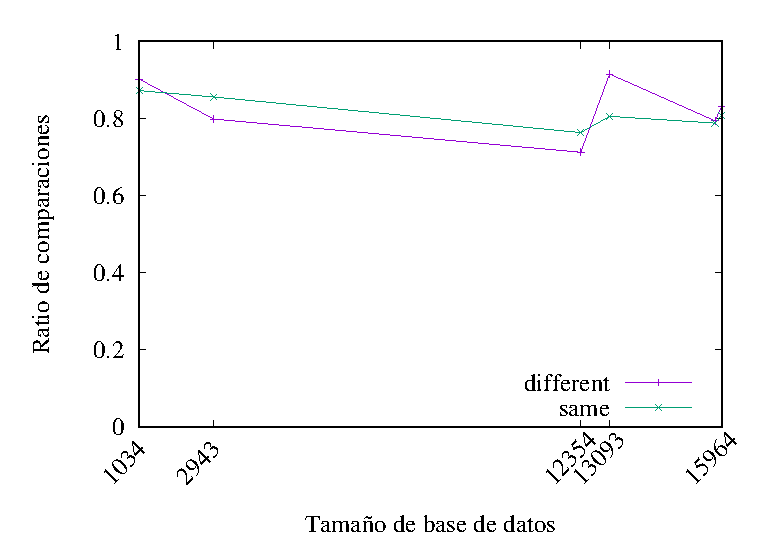
\includegraphics[width=71.5mm]{imagenes/same_vs_different/16p_incremental.eps}}
\subfigure[\scriptsize T\'ecnica de selecci\'on aleatoria]{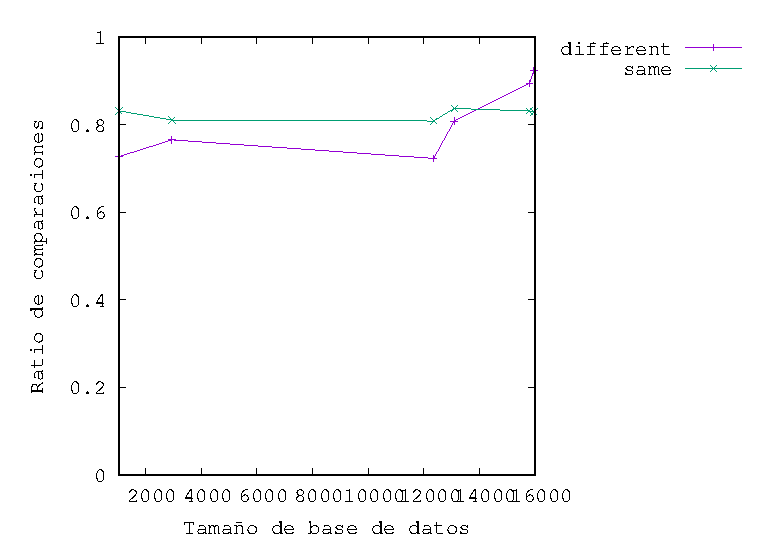
\includegraphics[width=71.5mm]{imagenes/same_vs_different/16p_random.eps}}
		\caption{\small Estrategia de selecci\'on para 16 pivotes: mismos pivotes vs diferentes}
		\label{fig:same-vs-diff-16Pivotes}
\end{figure}

\begin{figure}[tb]
\centering
\subfigure[\scriptsize T\'ecnica de selecci\'on incremental]{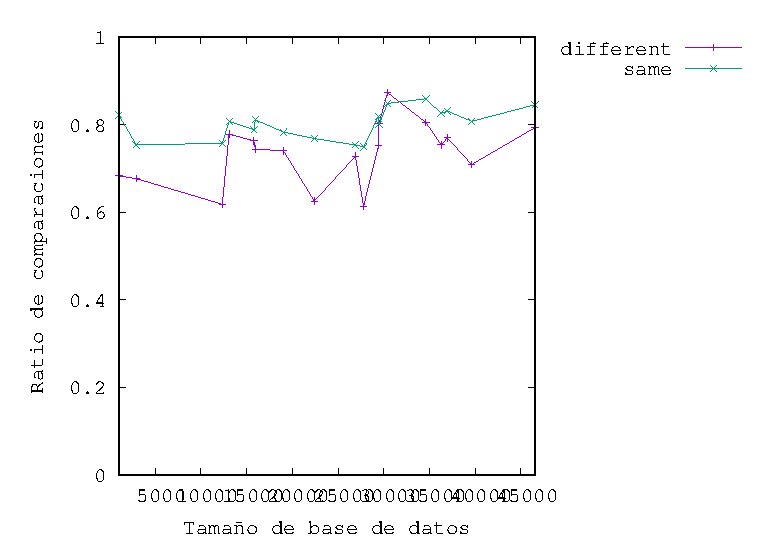
\includegraphics[width=71.5mm]{imagenes/same_vs_different/64p_incremental.eps}}
\subfigure[\scriptsize T\'ecnica de selecci\'on aleatoria]{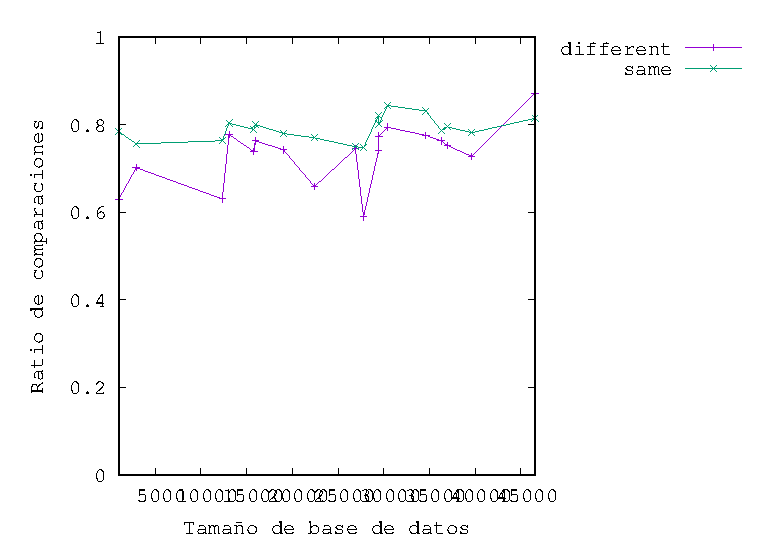
\includegraphics[width=71.5mm]{imagenes/same_vs_different/64p_random.eps}}
		\caption{\small Estrategia de selecci\'on para 64 pivotes: mismos pivotes vs diferentes}
		\label{fig:same-vs-diff-64Pivotes}
\end{figure}

\section{Ejecuci\'on experimental}

Se seleccion\'o al azar el 10\% de los elementos de cada una de las bases de datos para realizar las b\'usquedas. La cantidad total de b\'usquedas por rango realizadas fue: 339.899. Este valor incluye las b\'usquedas usadas para descartar la pol\'itica de selecci\'on \textit{Mismo grupo de pivotes para todas las categor\'ias } mencionada anteriormente.\\

En total se ejecutaron 276 experimentos. Esto es, 138 experimentos usando t\'ecnica de selecci\'on de pivotes aleatoria y 138 experimentos usando t\'ecnica de selecci\'on de pivotes incremental.\\

Los experimentos fueron ejecutados en una computadora port\'atil MacBook Pro, con un procesador 2,5 GHz Intel Core i7 y 16GB de memoria RAM.

\section{An\'alisis de resultados}

Vamos a presentar los resultados segmentados en cuatro grupos y analizaremos tres enfoques diferentes.\\

\subsection{Efecto de la cantidad de pivotes}


\begin{figure}[tb]
\centering
\subfigure[\scriptsize T\'ecnica de selecci\'on de pivotes aleatoria]{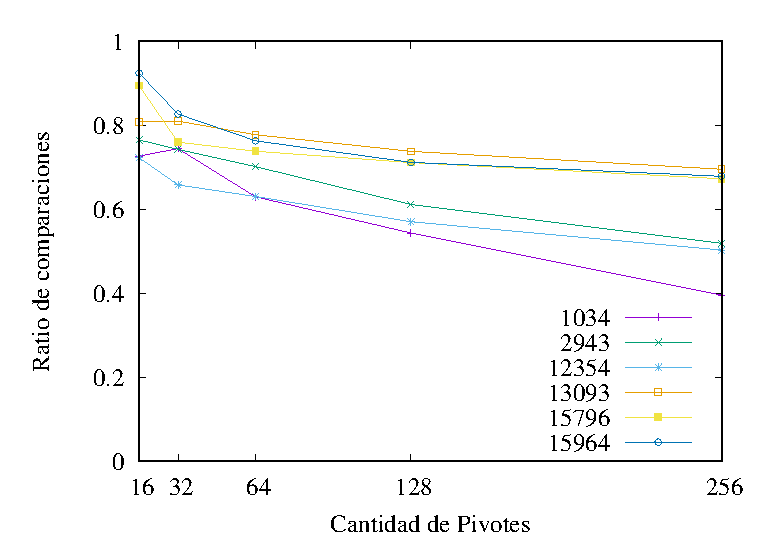
\includegraphics[width=71.5mm]{imagenes/efecto_pivotes/g1_random_ep.eps}}
\subfigure[\scriptsize T\'ecnica de selecci\'on de pivotes incremental]{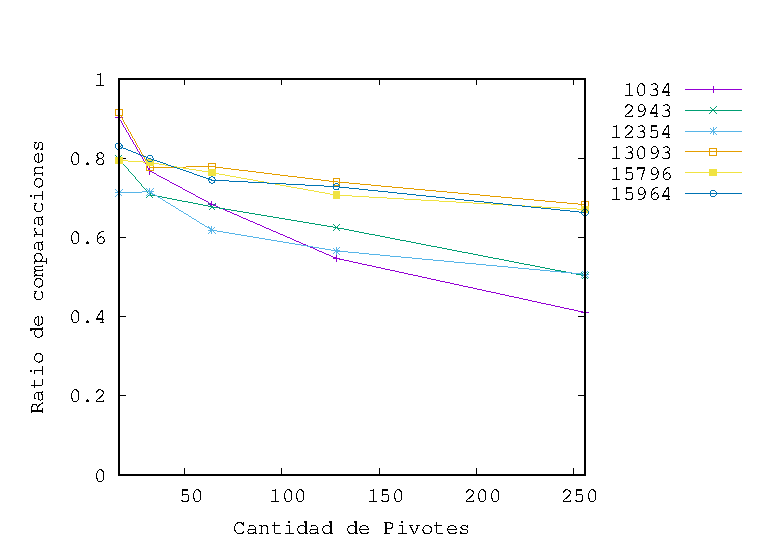
\includegraphics[width=71.5mm]{imagenes/efecto_pivotes/g1_incremental_ep.eps}}
		\caption{\small Grupo 1 - Efecto de la cantidad de pivotes sobre el ratio de comparaciones.}
		\label{fig:EP-g1}
\end{figure}

\begin{figure}[tb]
\centering
\subfigure[\scriptsize T\'ecnica de selecci\'on de pivotes aleatoria]{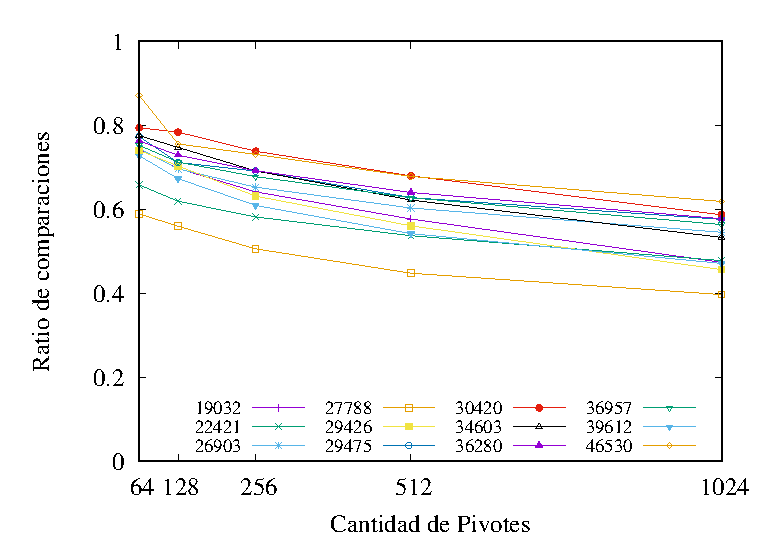
\includegraphics[width=71.5mm]{imagenes/efecto_pivotes/g2_random_ep.eps}}
\subfigure[\scriptsize T\'ecnica de selecci\'on de pivotes incremental]{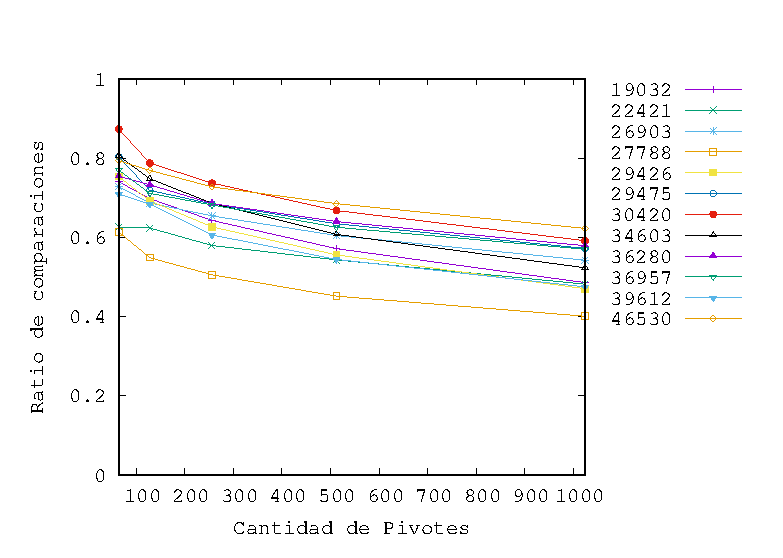
\includegraphics[width=71.5mm]{imagenes/efecto_pivotes/g2_incremental_ep.eps}}
		\caption{\small Grupo 2 - Efecto de la cantidad de pivotes sobre el ratio de comparaciones.}
		\label{fig:EP-g2}
\end{figure}

\begin{figure}[tb]
\centering
\subfigure[\scriptsize T\'ecnica de selecci\'on de pivotes aleatoria]{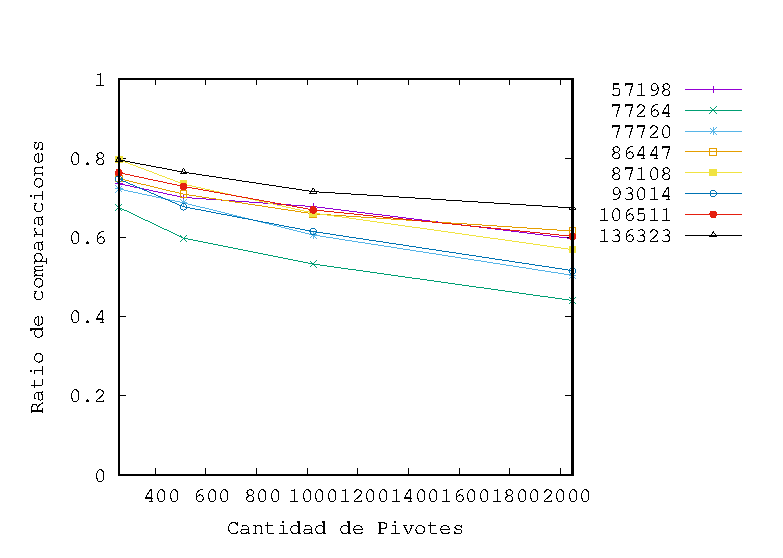
\includegraphics[width=71.5mm]{imagenes/efecto_pivotes/g3_random_ep.eps}}
\subfigure[\scriptsize T\'ecnica de selecci\'on de pivotes incremental]{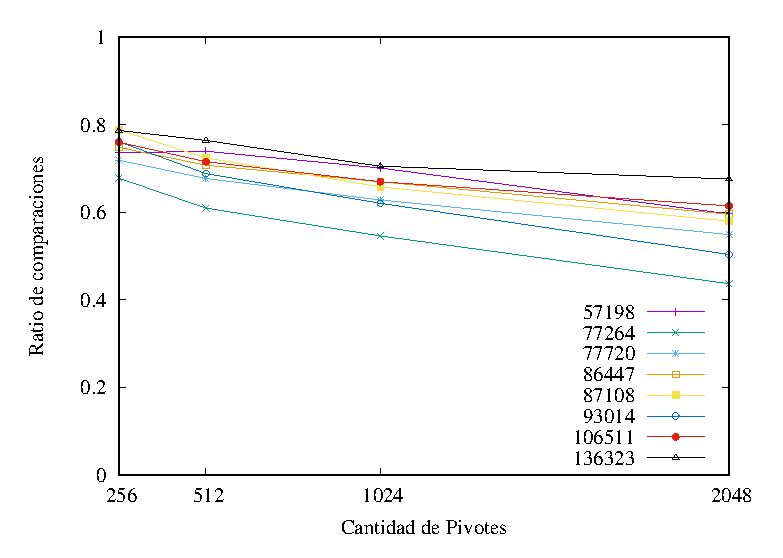
\includegraphics[width=71.5mm]{imagenes/efecto_pivotes/g3_incremental_ep.eps}}
		\caption{\small Grupo 3 - Efecto de la cantidad de pivotes sobre el ratio de comparaciones.}
		\label{fig:EP-g3}
\end{figure}

\begin{figure}[tb]
\centering	
\subfigure[\scriptsize T\'ecnica de selecci\'on de pivotes aleatoria]{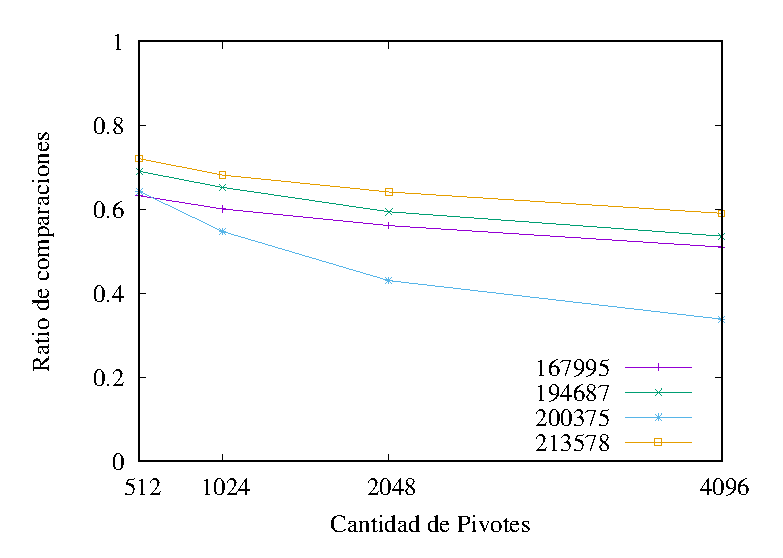
\includegraphics[width=71.5mm]{imagenes/efecto_pivotes/g4_random_ep.eps}}
\subfigure[\scriptsize T\'ecnica de selecci\'on de pivotes incremental]{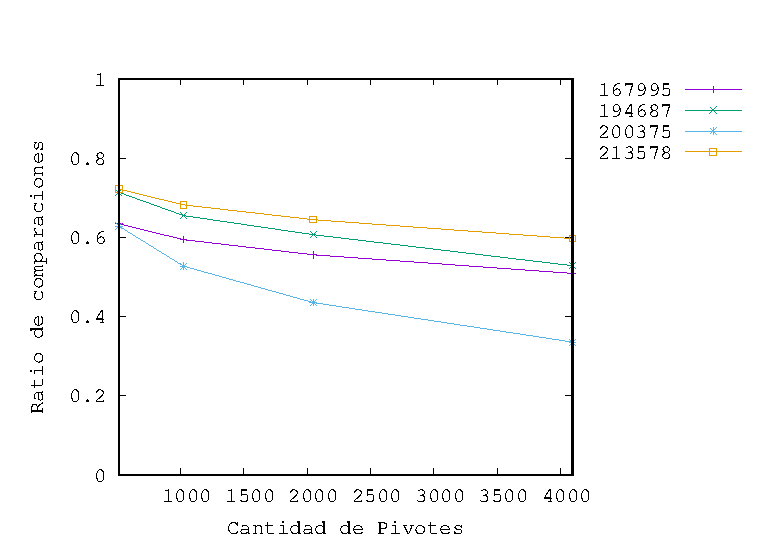
\includegraphics[width=71.5mm]{imagenes/efecto_pivotes/g4_incremental_ep.eps}}
		\caption{\small Grupo 4 - Efecto de la cantidad de pivotes sobre el ratio de comparaciones.}
		\label{fig:EP-g4}
\end{figure}

A continuaci\'on vamos a analizar el efecto de la cantidad de pivotes sobre el ratio de comparaciones para cada base de datos. Cada l\'inea representa una base de datos y su descripci\'on est\'a determinada por la cantidad de elementos que contiene, como puede observarse en las gr\'aficas.\\

En la figura \ref{fig:EP-g1}, observamos que tanto para selecci\'on de pivotes aleatoria (a) como para selecci\'on de pivotes incremental (b), para $16, 32, 64, 128$ y $256$ pivotes, a medida que aumenta el n\'umero de pivotes, el ratio de comparaciones disminuye. Tambi\'en vemos que las 3 bases de datos mas grandes tienen un comportamiento similar, es decir el ratio de comparaciones oscila entre $0,7$ y $0,93$ aproximadamente y para las 3 bases de datos mas chicas, oscila entre $0,4$ y $0,8$ aproximadamente.\\

En la figura \ref{fig:EP-g2}, observamos que para los pivotes $64, 128, 256, 512$ y $1024$ ambas t\'ecnicas de selecci\'on de pivotes se comportan de manera similar, a mayor n\'umero de pivotes, menor ratio de comparaciones. El ratio de comparaciones est\'a entre $0,6$ y $0,8$ para todas las bases de datos excepto la $27788$ que se encuentra entre $0,4$ y $0,6$.\\

En la figura \ref{fig:EP-g3}, observamos el mismo comportamiento que para los grupos 1 y 2. Para la mayor\'ia de las bases de datos y para ambas t\'ecnicas de selecci\'on, el ratio de comparaciones est\'a entre $0,6$ y $0,8$. Para la cantidad de pivotes de este grupo, $256, 512, 1024$ y $2048$, tambi\'en se cumple la tendencia de que a mayor n\'umero de pivotes menor ratio de comparaciones.\\

En la figura \ref{fig:EP-g4}, observamos que a medida que aumenta el n\'umero de pivotes el ratio de comparaciones disminuye, de manera similar al resto de los grupos. Tambi\'en vemos que 3 de las 4 bases de datos que estamos analizando, para los pivotes 512, 1024 y 2048; el ratio de comparaciones est\'a entre $0,6$ y $0,75$ aproximadamente y para 4096 pivotes, entre $0,5$ $0,6$.\\

A modo de resumen, analizando el efecto de la cantidad de pivotes en general para los cuatro grupos, vemos que cuando aumenta el n\'umero de pivotes decrementa el ratio de comparaciones pero las t\'ecnicas de selecci\'on aleatoria e incremental no muestran diferencias significativas entre s\'i.

\subsection{Efecto del tamaño de la base de datos}

\begin{figure}[tb]
\centering
\subfigure[\scriptsize T\'ecnica de selecci\'on de pivotes aleatoria]{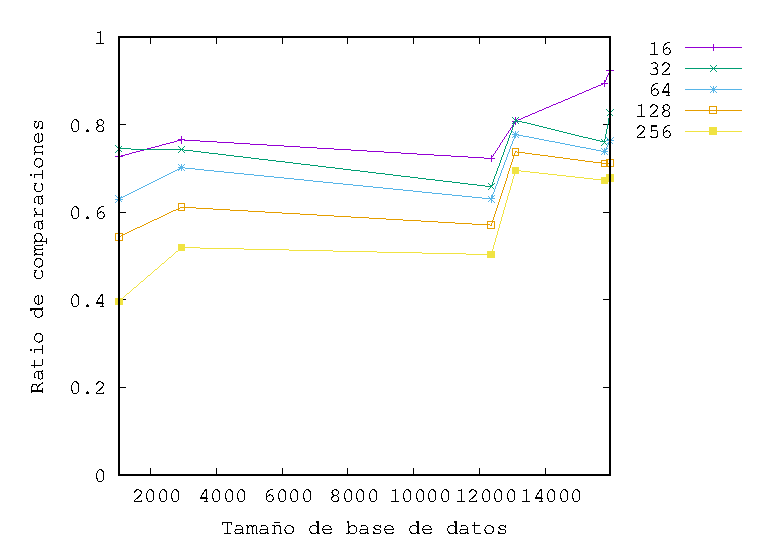
\includegraphics[width=71.5mm]{imagenes/efecto_db/g1_random_edb.eps}}
\subfigure[\scriptsize T\'ecnica de selecci\'on de pivotes incremental]{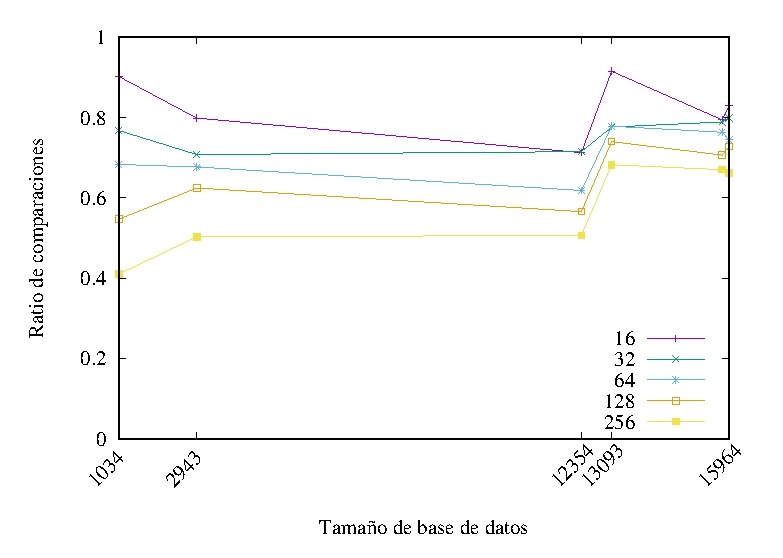
\includegraphics[width=71.5mm]{imagenes/efecto_db/g1_incremental_edb.eps}}
		\caption{\small Grupo 1 - Efecto del tamaño de la base de datos sobre el ratio de comparaciones por pivotes.}
		\label{fig:EDB-g1}
\subfigure[\scriptsize T\'ecnica de selecci\'on de pivotes aleatoria]{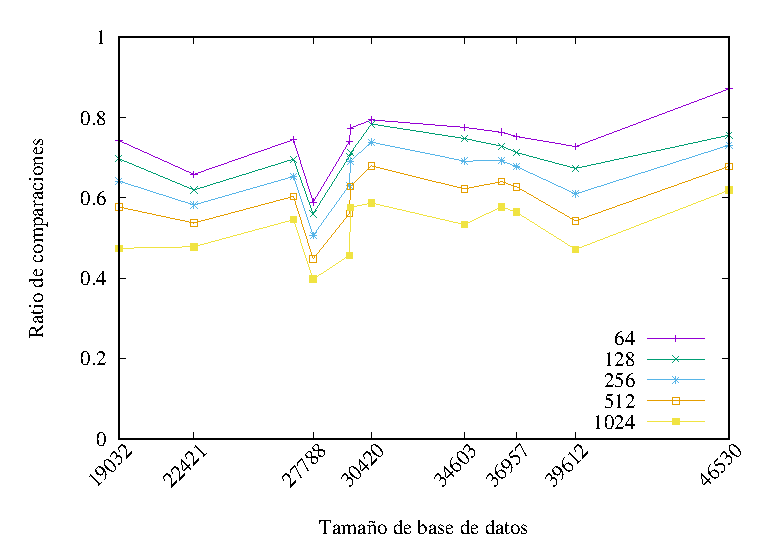
\includegraphics[width=71.5mm]{imagenes/efecto_db/g2_random_edb.eps}}
\subfigure[\scriptsize T\'ecnica de selecci\'on de pivotes incremental]{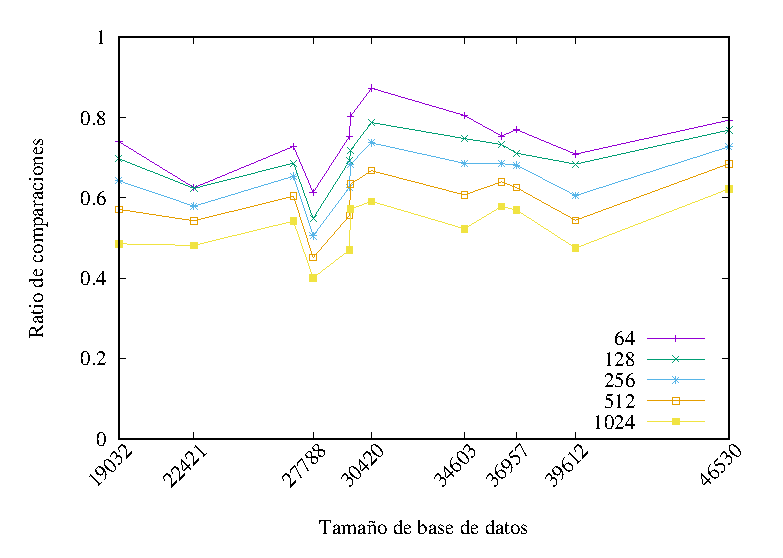
\includegraphics[width=71.5mm]{imagenes/efecto_db/g2_incremental_edb.eps}}
		\caption{\small Grupo 2 - Efecto del tamaño de la base de datos sobre el ratio de comparaciones por pivotes.}
		\label{fig:EDB-g2}
\end{figure}

\begin{figure}[tb]
\centering
\subfigure[\scriptsize T\'ecnica de selecci\'on de pivotes aleatoria]{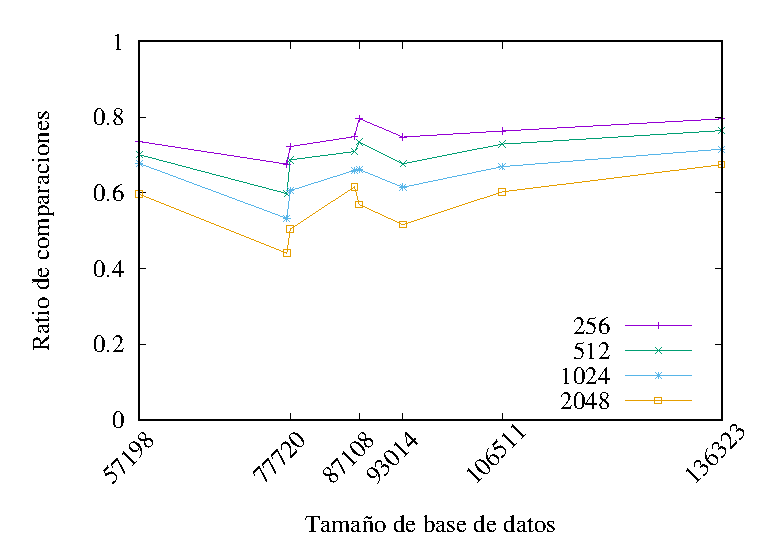
\includegraphics[width=71.5mm]{imagenes/efecto_db/g3_random_edb.eps}}
\subfigure[\scriptsize T\'ecnica de selecci\'on de pivotes incremental]{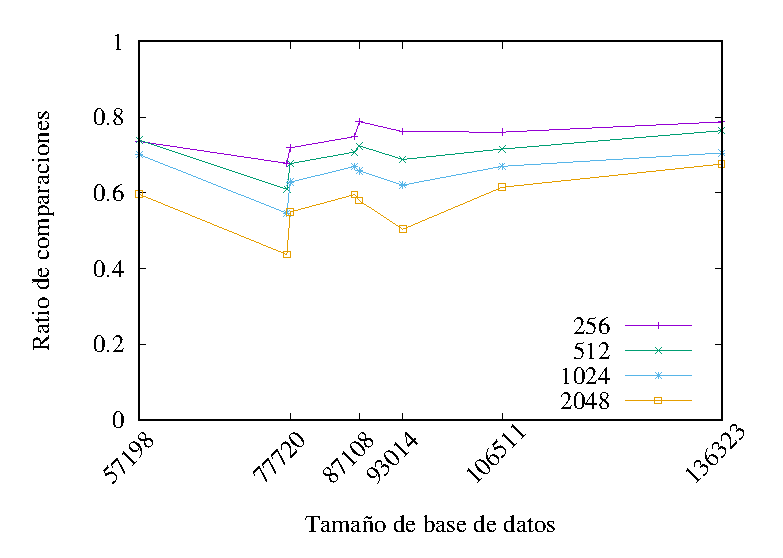
\includegraphics[width=71.5mm]{imagenes/efecto_db/g3_incremental_edb.eps}}
		\caption{\small Grupo 3 - Efecto del tamaño de la base de datos sobre el ratio de comparaciones por pivotes.}
		\label{fig:EDB-g3}
\end{figure}

\begin{figure}[tb]
\centering
\subfigure[\scriptsize T\'ecnica de selecci\'on de pivotes aleatoria]{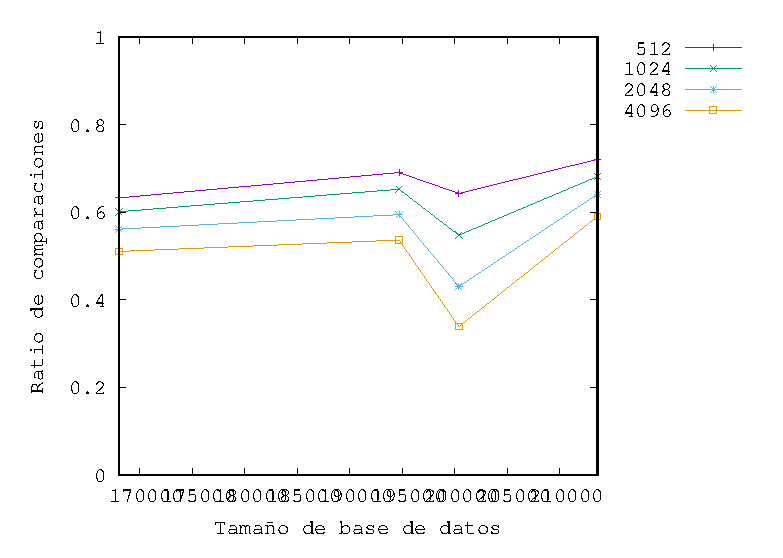
\includegraphics[width=71.5mm]{imagenes/efecto_db/g4_random_edb.eps}}
\subfigure[\scriptsize T\'ecnica de selecci\'on de pivotes incremental]{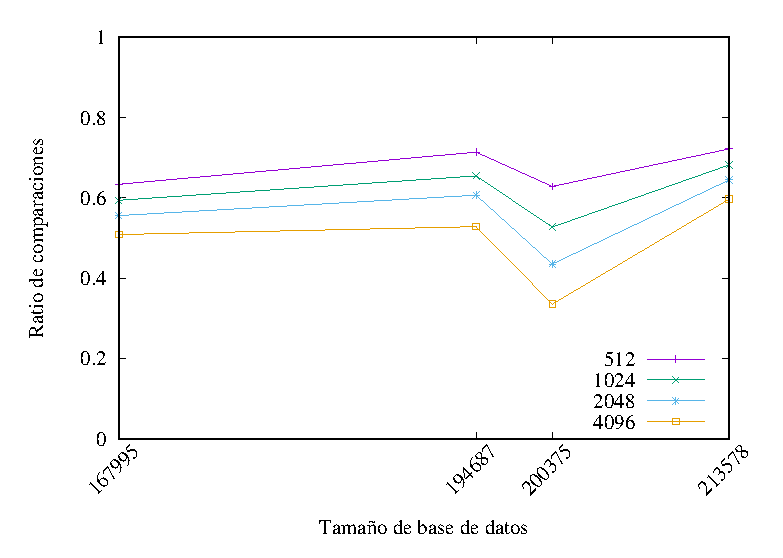
\includegraphics[width=71.5mm]{imagenes/efecto_db/g4_incremental_edb.eps}}
		\caption{\small Grupo 4 - Efecto del tamaño de la base de datos sobre el ratio de comparaciones por pivotes.}
		\label{fig:EDB-g4}
\end{figure}
 
A continuaci\'on vamos a analizar cual es el efecto del tama\~no de las bases de datos sobre el ratio de comparaciones por pivotes. Las l\'ineas de las graficas representan el n\'umero de pivotes con los que se ejecutaron las b\'usquedas.\\

En la figura \ref{fig:EDB-g1} presentamos los resultados para el grupo 1; donde el rango del tama\~no de las bases de datos varía de $1034$ a $15964$ objetos y la cantidad de pivotes utilizados es $16, 32, 64, 128$ y $256$.\\

Para la t\'ecnica de selecci\'on de pivotes aleatoria (a), en la base de datos mas chica, el ratio de comparaciones esta entre $0,4$ y $0,8$ y para las bases de datos m\'as grandes, entre $0,7$ y $0,9$. Por otro lado, si miramos la gr\'afica para $256$ pivotes podemos observar que para la base de datos mas chica el ratio de comparaciones es $0,4$ y a medida que crece en tama\~no de la base de datos el ratio de comparaciones tambien aumenta ($0,7$ en las bases de datos mas grandes).\\

Para la t\'ecnica de selecci\'on de pivotes incremental (b), el comportamiento es similar, a menor cantidad de pivotes, mayor ratio de comparaciones.\\

En la figura \ref{fig:EDB-g2}, donde el tama\~no de las bases de datos van desde $19032$ a $46530$ elementos y los pivotes usados son $64, 128, 256, 512$ y $1024$, el ratio de comparaciones no tiene mucha variabilidad desde la base de datos mas chica a las mas grande.\
Por ejemplo: para t\'ecnica de selecci\'on de pivotes aleatoria, 512 pivotes y una base de datos de 19.000 elementos el ratio de comparaciones es $0,58$ aproximadamente y para una base de datos de 46.000 elementos, el ratio es $0,67$. Estos valores son similares para el caso de t\'ecnica de selecci\'on de pivotes incremental.\\

A nivel general, para t\'ecnica de selecci\'on de pivotes aleatoria, podemos ver que para la base de datos mas chica, el ratio de comparaciones varia entre $0,49$ y $0,79$; y para las bases de datos mas grande, entre $0,6$ y $0,84$. Para la t\'ecnica de selecci\'on de pivotes incremental los rangos de ratios de comparaciones estan entre $[0,5 - 0,77]$ y $[0,61 - 0,79]$. \\

Para las figuras \ref{fig:EDB-g3} y \ref{fig:EDB-g4}, donde se muestran los grupos 3 y 4 respectivamente, el comportamiento es similar al de los grupos antes mencionados.\\

A medida que el tama\~no de las bases de datos aumenta, el ratio de comparaciones tambi\'en crece, aunque la variabilidad de este \'ultimo es muy baja. Esto es similar para ambas t\'ecnicas de selecci\'on de pivotes.

\subsection{Comparaci\'on de las t\'ecnicas de selecci\'on de pivotes}

En esta secci\'on vamos a comparar las t\'ecnicas de selecci\'on de pivotes aleatoria e incremental, usando como m\'etrica el n\'umero de evaluaciones de distancia para cada unos de los grupos de pivotes elegidos. Se realizaron las comparaciones para todas las bases de datos con las que trabajamos (30) pero a continuaci\'on s\'olo analizaremos la base de datos de mayor tama\~no de cada uno de los grupos que mencionamos anteriormente, el resto se adjuntan en el Anexo \ref{anexo.A}.\\

Para el grupo 1, figura \ref{fig:ETS-1}(a), observamos que para una base de datos de aproximadamente 16.000 elementos, usando la t\'ecnica de selecci\'on incremental se realizan menos evaluaciones de distancia que la t\'ecnica de selecci\'on aleatoria para todos los grupos de pivotes, excepto para 128 pivotes. Tambi\'en se puede observar que la diferencia entre ambas t\'ecnicas es amplia.\\

Para el grupo 2, figura \ref{fig:ETS-1}(b), para una base de datos de aproximadamente 45.000 elementos, la t\'ecnica de selecci\'on incremental es mejor solo en dos grupos de pivotes, 64 y 256. Para los grupos de pivotes de 128, 512 y 1024, la t\'ecnica de selecci\'on aleatoria realiza menos evaluaciones de distancia que la incremental. Tambi\'en se puede observar que a partir del grupo de pivotes 256, la diferencia en la cantidad de evaluaciones de distancia no es tan grande entre ambas t\'ecnicas.\\

Para el grupo 3, figura \ref{fig:ETS-2}(a), con una base de datos de aproximadamente 136.000 elementos, la t\'ecnica de selecci\'on incremental en general realiza menor cantidad de evaluaciones de distancia, salvo para 2048 pivotes. Para este ultimo grupo de pivotes, la t\'ecnica de selecci\'on aleatoria esta por debajo de incremental pero solo por una m\'inima diferencia.\\

Para el grupo 4, figura \ref{fig:ETS-2}(b), con una base de datos de aproximadamente 213.000 elementos, en general, la t\'ecnica de selecci\'on aleatoria realiza menos evaluaciones de distancia que la t\'ecnica de selecci\'on incremental, aunque dicha diferencia es casi imperceptible (excepto para 4096, donde la diferencia es mas marcada).\\


\begin{figure}[tb]
\centering
\subfigure[\scriptsize Grupo 1]{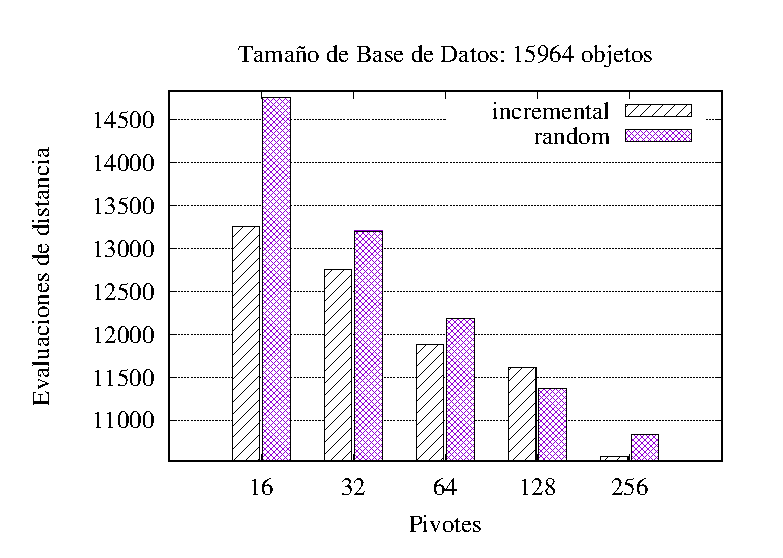
\includegraphics[width=71.5mm]{imagenes/random_vs_incremental/g1_15964.eps}}
\subfigure[\scriptsize Grupo 2]{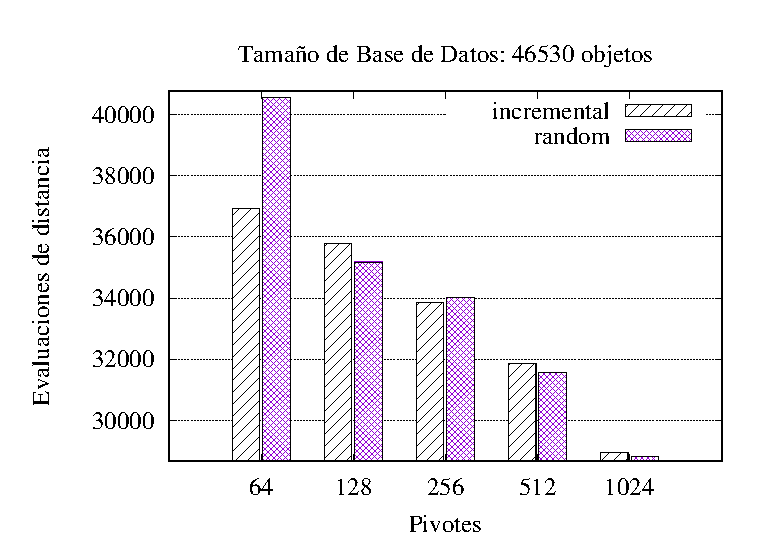
\includegraphics[width=71.5mm]{imagenes/random_vs_incremental/g2_46530.eps}}
\caption{\small Comparaci\'on de las t\'ecnicas de selecci\'on de pivotes random vs. incremental.}
\label{fig:ETS-1}
\end{figure}
\begin{figure}[tb]
\centering
\subfigure[\scriptsize Grupo 3]{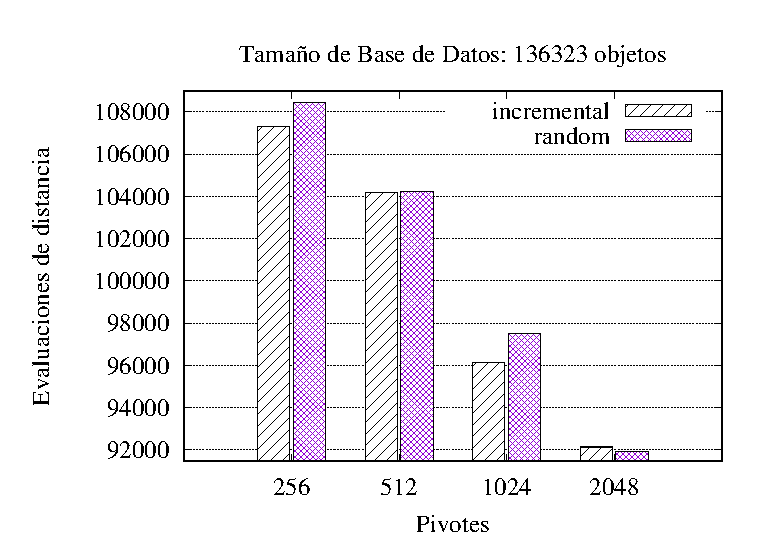
\includegraphics[width=71.5mm]{imagenes/random_vs_incremental/g3_136323.eps}}
\subfigure[\scriptsize Grupo 4]{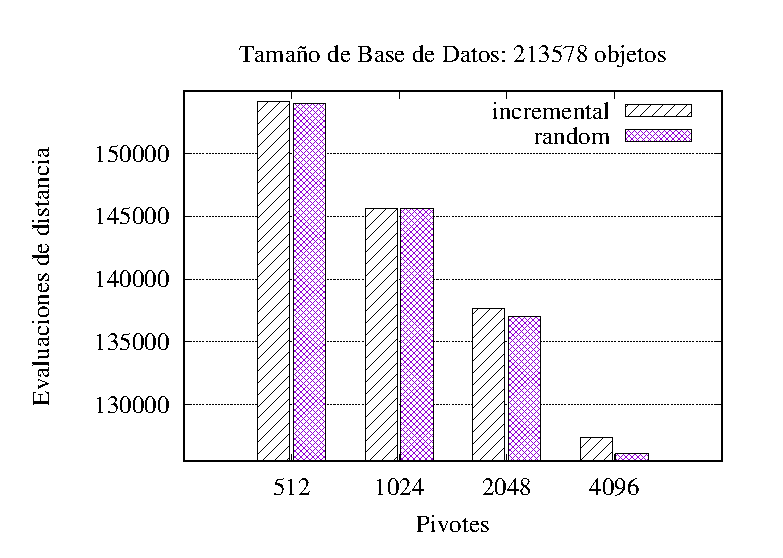
\includegraphics[width=71.5mm]{imagenes/random_vs_incremental/g4_213578.eps}}
\caption{\small Comparaci\'on de las t\'ecnicas de selecci\'on de pivotes random vs. incremental.}
\label{fig:ETS-2}

\end{figure}

Como conclusi\'on general, se puede observar que la t\'ecnica de selecci\'on aleatoria ejecuta menos evaluaciones de distancia, aunque la diferencia con la selecci\'on incremental no es altamente significativa.\\

En la gran variedad de los trabajos existentes sobre el tema se ha demostrado que la t\'ecnica de selecci\'on incremental funciona mejor que la aleatoria, pero como podemos observar de los resultados de los experimentos realizados, \'esta afirmaci\'on no se cumple para las bases de datos utilizadas. Para encontrar la raz\'on del comportamiento observado, procedimos a realizar un an\'alisis emp\'irico de la distribuci\'on de los elementos de las diferentes categor\'ias. Dicho an\'alisis se presenta en la siguiente secci\'on.


\section{Histogramas de distancia}
 
Los resultados obtenidos de los experimentos, en conjunci\'on con el excesivo tiempo de ejecuci\'on de los algoritmos de b\'usqueda fueron un indicativo de que pod\'iamos estar ante un espacio de alta dimensionalidad.\\

Dado que cada base de datos es un universo completamente distinto y que en todos los casos vimos el mismo comportamiento, decidimos realizar el c\'alculo de los histogramas de distancia para todas las bases de datos. En esta secci\'on solo analizaremos los histogramas de las categor\'ias con mayor cantidad de elementos de cada grupo, pero un listado completo puede encontrarse en el Anexo \ref{anexo.B}.\\\\

En la figuras \ref{fig:HF1} y \ref{fig:HF2} se puede observar como se concentran los elementos, asemejandose a un histograma de alta dimensionalidad como vimos en la figura \ref{dim1} (p\'agina \pageref{dim1}).\\

Esto indica que a medida que los elementos se encuentran mas concentrados alrededor de su media, disminuye la cantidad de elementos que pueden ser descartados por el proceso de b'usqueda. Esto es, aumenta la cantidad de comparaciones con elementos de base de datos.\\

Si analizamos nuevamente las figuras \ref{fig:EP-g4} y \ref{fig:EDB-g4} que muestran el efecto de la cantidad de pivotes y el efecto del tama\~no de la base de datos respectivamente, para ambos casos, independientemente de la t\'ecnica de selecci\'on, vemos que el ratio de comparaciones para 4096 pivotes o para la base de datos m\'as grande ronda el 0,6 lo cual es equivalente al 60\%. Esto quiere decir que ante una b\'usqueda, el algoritmo descarta menos de la mitad de los elementos de la base de datos.\\

Como s\'intensis, vemos en general que ninguna de las t\'ecnicas de selecci\'on ofrece una opci\'on eficiente, ya que el porcentaje de comparaciones con los elementos de la base de datos es elevado para ambas t\'ecnicas.\\

\begin{figure}[tb]
\centering
\subfigure{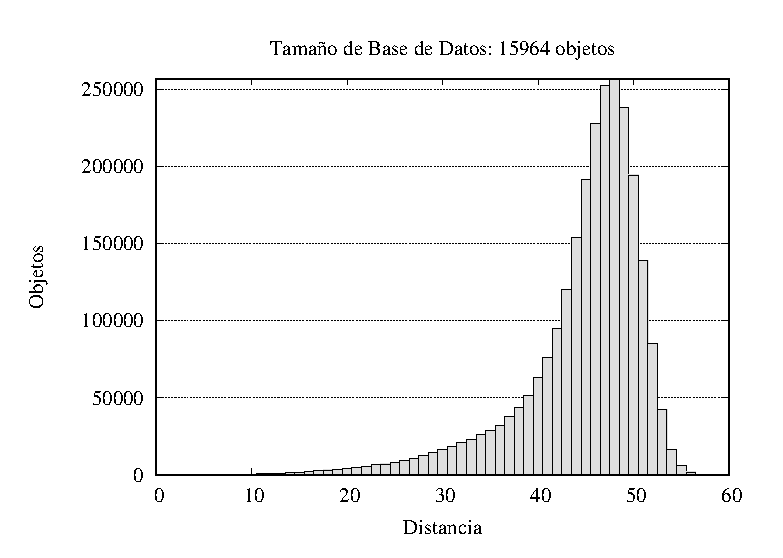
\includegraphics[width=71.5mm]{imagenes/histogramas/31928_items.eps}}
\subfigure{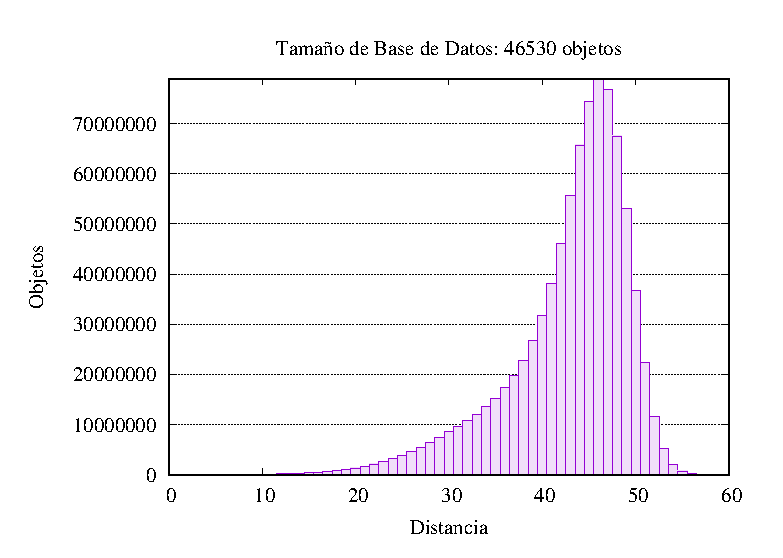
\includegraphics[width=71.5mm]{imagenes/histogramas/93060_items.eps}}
		\caption{\small Histogramas de frecuencia de la base de datos m\'as grandes del grupo 1 (izquierda) y del grupo 2 (derecha).}
		\label{fig:HF1}
		
\subfigure{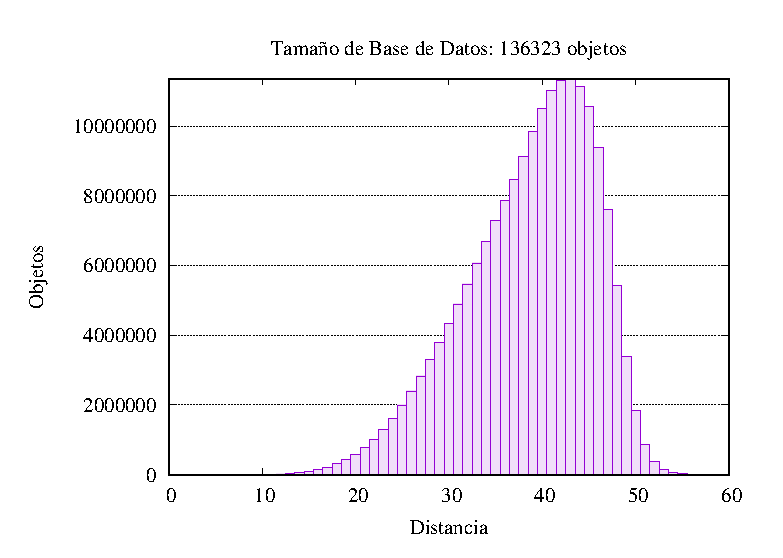
\includegraphics[width=71.5mm]{imagenes/histogramas/272646_items.eps}}
\subfigure{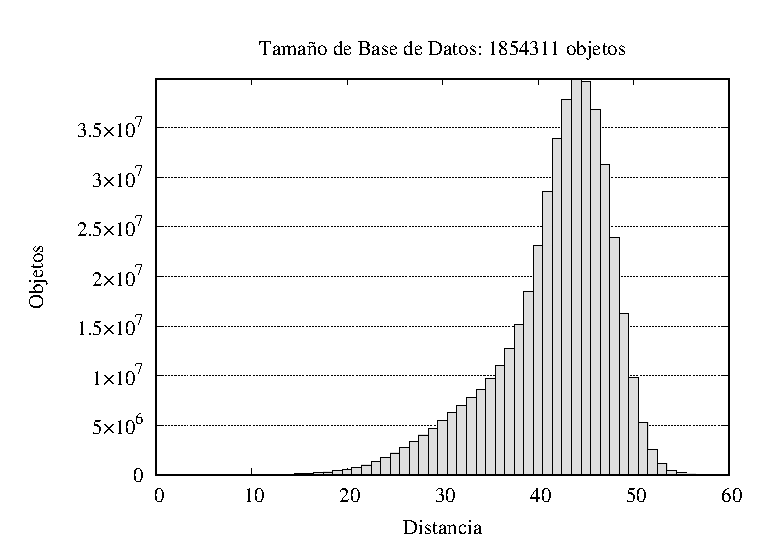
\includegraphics[width=71.5mm]{imagenes/histogramas/1854311_items.eps}}
	\caption{\small Histogramas de frecuencia de la base de datos m\'as grandes del grupo 3 (izquierda) y del grupo 4 (derecha).}
		\label{fig:HF2}
\end{figure}


\section{B\'usqueda de los k-vecinos}

Como \'ultimo paso en la ejecuci\'on de experimentos, definimos realizar la b\'usqueda de los \textit{k-vecinos} con $k=5$, para la base de datos con mayor cantidad de elementos de cada grupo, utilizando la mayor cantidad de pivotes del mismo y la estrategia de selecci\'on aleatoria.\\

Esta clase de experimento nos dar\'ia un indicio del comportamiento en general de nuestro sistema de recomendaci\'on.\\

Para las b\'usquedas de los \textit{k-vecinos} se utiliz\'o el mismo conjunto de items que para el resto de los experimentos, es decir, 10\% de los elementos pertenecientes a cada categor\'ia, seleccionados al azar.\\

\begin{table}[H]
\begin{center}
\begin{tabular}{|c|c|c|c|}
\hline \multirow{2}{5cm}{\small Tama\~no de base de datos}
& \multicolumn{3}{p{4cm}|}
{\centering \small Ratio de comparaciones}\tabularnewline \cline{2-4}
& \multicolumn{1}{p{1.2cm}|}
{\centering \small Prom.}
& \multicolumn{1}{p{1.2cm}|}
{\centering \small Max.}
& \multicolumn{1}{p{1.2cm}|}
{\centering \small Min.}
\tabularnewline \hline
\hline \small 15964 & 0.83845 & 1 & 0.00031 \\ \hline
\hline \small 46530 & 0.78821 & 1 & 0.00011 \\ \hline
\hline \small 136323 & 0.84512 & 1 & 0.00012 \\ \hline
\hline \small 213578 & 0.76582 & 1 & 0.00004 \\ \hline
\end{tabular}
\caption{\small Resultados de la b\'usqueda de los \textit{k-vecinos} con $k=5$.}
\label{tabla:knn}
\end{center}
\end{table}



En la tabla \ref{tabla:knn} presentamos los resultados obtenidos de dichos experimentos. Como podemos observar, el promedio del ratio de comparaciones fue superior a 0,7, es decir que para obtener los resultados de la b\'usqueda el algoritmo realizó m\'as del 70\% de evaluaciones de distancia respecto del total de elementos de la base de datos.\\

Otro dato de inter\'es a tener en cuenta es la gran variabilidad entre el m\'aximo y el m\'inimo del ratio de comparaciones, el cual es un indicador de que para algunas pocas b\'usquedas el algoritmo funcion\'o con \'optima eficiencia, pero para otras se comport\'o de la misma manera que una b\'usqueda secuencial.\\

Claramente, el comportamiento sub\'optimo del algoritmo de b\'usqueda se debe a la alta dimensionalidad del espacio m\'etrico representado por cada una de las categor\'ias.